% ── Detecting Coordinated Wallet Behaviour on Solana ──
\documentclass[10pt,journal]{IEEEtran}

% ── Packages ───────────────────────────────────────────────────────
\usepackage[T1]{fontenc}
\usepackage{amsmath,amssymb}
\usepackage{booktabs}
\usepackage{graphicx}
\usepackage[font=small,labelfont=bf]{caption}
\usepackage{cite}
\usepackage[colorlinks=false]{hyperref}
\usepackage{microtype}
\usepackage{multirow}
\usepackage{enumitem}
\setlist{nosep,leftmargin=1.2em}
\usepackage[ruled,vlined,linesnumbered]{algorithm2e}
\SetAlFnt{\small}

% Tight float spacing
\setlength{\textfloatsep}{6pt plus 1pt minus 1pt}
\setlength{\floatsep}{6pt plus 1pt minus 1pt}
\setlength{\intextsep}{4pt plus 1pt minus 1pt}
\setlength{\abovecaptionskip}{3pt}
\setlength{\belowcaptionskip}{1pt}
\setlength{\abovedisplayskip}{6pt plus 2pt minus 2pt}
\setlength{\belowdisplayskip}{6pt plus 2pt minus 2pt}

% ── Title ──────────────────────────────────────────────────────────
\title{Zero Features, Full Signal: Topology-Driven\\
Coordination Analysis in Meme-Token Markets}
\author{Andrea Nardello
\thanks{COMP0162 Advanced Machine Learning in Finance, University
College London, 2025/26.}}

\begin{document}
\maketitle

% ── Abstract ───────────────────────────────────────────────────────
\begin{abstract}
Coordinated wallet groups drive the majority of manipulation in
Solana's meme-token markets, yet existing detection methods rely on
hand-crafted token-level features that cannot capture the relational
structure of coordination itself. We model the ecosystem as a
heterogeneous wallet--token interaction graph and investigate how much
of the information needed to identify and anticipate coordinated
manipulation is encoded in interaction topology alone.
\textit{First}, a featureless heterogeneous GAT using only learnable type
embeddings \emph{detects} coordination with
AUC\,=\,0.867\,[0.852,\,0.882], outperforming five tabular
baselines operating on 116~engineered features (best: Random Forest,
0.855). \textit{Second}, a Bochner-encoded temporal extension
\emph{predicts} where coordinated wallets will target next, achieving
MRR\,=\,0.490 and Hits@10\,=\,0.952 ($2.7\times$ random), outperforming
EdgeBank and popularity heuristics that score below chance.
\textit{Third}, unsupervised clustering of the learned embeddings
reveals three coordination \emph{archetypes}, bundled bot operators,
organic retail, and loosely synchronised groups, without any explicit
supervision on wallet types. An early-detection analysis shows that
topological signal requires approximately three days of accumulated
interactions to match feature-based methods, establishing the two
modalities as complementary for staged monitoring.
\end{abstract}

% ====================================================================
\section{Introduction}
\label{sec:intro}
% ====================================================================

Coordination is the organising principle behind manipulation in
meme-token markets. On Solana, platforms such as Pump.fun launch
upwards of 50{,}000 tokens per day, collectively generating over
\$5\,billion in daily DEX volume, and a majority are associated
with orchestrated activity: insider wallets inflate early volume to
attract retail capital, then withdraw
liquidity~\cite{hu2026memetrans}. The MemeTrans dataset documents
over 41{,}000 such tokens, of which approximately 79\,\% are labelled
high-risk based on return ratios. What makes these schemes effective
is not any single wallet's behaviour but the \emph{coordination}
among wallets: same-transaction bundling, sub-second co-trading
across multiple tokens, and hub-and-spoke subgraph formation. These
are inherently relational signals that per-token aggregate statistics
can only approximate.

Graph topology captures coordination in a way that token-level
features cannot. Coordinated clusters participate across
\emph{multiple} tokens, and a graph representation preserves the full
neighbourhood structure, capturing who traded what, when, and alongside
whom, enabling detection of coordination patterns that persist across
tokens and across time.

Prior work exists along three separate strands that have not yet been
integrated. On Solana, MemeTrans~\cite{hu2026memetrans} engineers 122
features from on-chain data and applies gradient-boosted trees;
SolRugDetector~\cite{chen2026solrugdetector} compiles over 76{,}000
rug-pull tokens from on-chain transaction patterns; and
Alizadeh and Khabbazian~\cite{alizadeh2025solana} analyse Solana NFT
graph structure without GNNs. None of these Solana-specific works
employ graph neural networks or temporal message passing.

On Ethereum, TokenScout~\cite{wu2024tokenscout} and
RugScreener~\cite{wu2025rugscreener} apply temporal GNNs to token
fraud, while Mazorra~et~al.~\cite{mazorra2022donotrug} provide an
early ML baseline. Weber~et~al.~\cite{weber2019elliptic} applied GCNs
to Bitcoin, and Li~et~al.~\cite{li2022blockchain_survey} survey
blockchain GNN anomaly detection. All rely on attributed graphs with
substantial node features.

A parallel line of work develops temporal GNN
primitives: TGAT~\cite{xu2020tgat} introduced Bochner time encodings,
TGN~\cite{rossi2020tgn} combined memory with temporal attention, and
Poursafaei~et~al.~\cite{poursafaei2022edgebank} established rigorous
evaluation protocols for dynamic link prediction.

Despite this body of work, three strands remain disconnected: no
prior study applies temporal GNNs to Solana meme-token coordination,
no study asks whether topology alone, without hand-crafted
features, suffices for risk detection, and no study formulates
wallet-token interaction prediction as temporal link prediction on
blockchain graphs.

We address this gap with a single research question: \emph{how much
of the information needed to identify and anticipate coordinated
manipulation is encoded in wallet--token interaction topology,
independent of hand-crafted features?} We answer under three aspects:
\begin{enumerate}[label=(\roman*)]
\item \textit{Detection.} Graph topology \emph{detects} coordination:
  a featureless HeteroGAT achieves AUC\,=\,0.867, exceeding the best
  tabular baseline (0.855) that operates on 116 engineered features.
\item \textit{Prediction.} Graph topology \emph{predicts} where
  coordinators will target next: a temporal extension achieves
  MRR\,=\,0.490 for next-token prediction.
\item \textit{Characterisation.} Topology reveals coordination
  \emph{archetypes}: unsupervised HDBSCAN
  clustering~\cite{mcinnes2017hdbscan} discovers bundled bot
  operators, organic retail, and loosely synchronised groups from
  embeddings alone.
\end{enumerate}

% ====================================================================
\section{Methodology}
\label{sec:method}
% ====================================================================

\subsection{Problem Formulation}
\label{sec:problem}

Let $\mathcal{G}=(\mathcal{V},\mathcal{E})$ be a heterogeneous graph
with node types $\mathcal{T}=\{\texttt{token},\texttt{wallet}\}$ and
edge types $\mathcal{R}=\{$\texttt{trade}, \texttt{reverse\_trade},
\texttt{co\_trade}, \texttt{same\_tx}$\}$. Each token node $\tau$ has a
binary label $y_\tau\in\{0,1\}$ indicating high-risk status. The
co-trading and same-transaction edges encode two complementary facets
of coordination: implicit synchronisation (wallets independently
arriving at the same tokens within seconds) and explicit bundling
(wallets transacting within the same atomic on-chain operation).

We study coordination through two complementary tasks.
\textit{Task~1 (Retrospective detection):}
Given $\mathcal{G}$ and labels on the training split, predict
$\hat{y}_\tau$ for tokens in the test split, identifying tokens
whose trading activity bears the structural fingerprint of coordination.
\textit{Task~2 (Prospective prediction):}
Given a sequence of timestamped interactions
$\{(w_i,\tau_j,t_{ij})\}_{t_{ij}\leq t_q}$, predict which token $\tau$
wallet $w$ will interact with at time $t>t_q$, forecasting where
coordinated groups will converge next.

\subsection{Data and Graph Construction}
\label{sec:data}

We draw from the MemeTrans dataset~\cite{hu2026memetrans}, which
catalogues meme-token activity on Solana's Pump.fun launchpad. The
dataset provides per-token features (holder concentration, price
dynamics, trading volume statistics) and a three-class risk label
(\texttt{high}, \texttt{medium}, \texttt{low}) derived from return
ratios; we binarise this as
$y_\tau{=}1$ for \texttt{high} and $y_\tau{=}0$ otherwise, following
the original authors' primary partition. We extract a three-week
subset (December 9--29, 2024) comprising 65.5\,million transactions
queried from Google BigQuery's Solana public dataset and split
chronologically: week~50 (Dec~9--15) for training, week~51
(Dec~16--22) for validation, week~52 (Dec~23--29) for testing. Each
split builds an independent graph to prevent temporal
leakage~\cite{poursafaei2022edgebank}.
Table~\ref{tab:data} reports split statistics.

\smallskip\textbf{Exploratory analysis.}
The label distribution is heavily skewed: approximately 79\,\% of
labelled tokens are classified as high-risk across all three splits
(Table~\ref{tab:data}), with a stable ratio of ${\sim}$3.7{:}1 that
confirms the prevalence of manipulation on Pump.fun. Weekly
transaction volume is stable (${\sim}20$--$23$M per week), as are
active wallet counts ($42$--$46$K) and edge counts, indicating that
the three-week window captures a stationary regime of market activity
rather than a transient event.

The bipartite degree distribution reveals a counter-intuitive
asymmetry: \emph{low-risk} tokens attract substantially more wallets
(median in-degree ${\sim}$1{,}174 in training) than high-risk tokens
(median ${\sim}$380). Legitimate tokens accumulate organic trading
volume over their lifetime, whereas coordinated pump-and-dump tokens
exhibit intense but concentrated activity from a smaller set of
wallets before liquidity is withdrawn. This inversion means that raw
wallet count is not a reliable risk indicator---coordination
\emph{structure} (who trades alongside whom) matters more than
coordination \emph{volume}, motivating the graph-based approach.
Wallet out-degree is right-skewed: the median active wallet trades 29
distinct tokens (the minimum is 20 by construction), while the 95th
percentile reaches ${\sim}$105 tokens and the most active wallet
trades over 2{,}600. This heavy tail captures the most prolific
coordinators, whose trading breadth generates the densest co-trading
subgraphs.

\smallskip\textbf{Data cleaning and preprocessing.}
We retain only \emph{active} wallets, defined as those trading
$\geq$20 distinct tokens. This threshold represents a
coverage--precision trade-off: a stricter filter ($\geq$50 tokens)
yields AUC\,=\,0.896 on a denser subgraph but retains only
${\sim}$1.7\,\% of wallets, discarding those involved in
narrowly-targeted campaigns; lowering the threshold below 20 admits
wallets whose co-trading edges reflect chance overlap rather than
systematic coordination. We select $\geq$20 as the operating point
that maximises population coverage (${\sim}$4\,\% of wallets,
responsible for the majority of inter-token coordination) while
preserving structural distinctiveness. MemeTrans provides 122 raw
features per token (holder Gini coefficients, top-$k$ holder
percentages, price and volume statistics, temporal indicators); after
removing identifier columns and label-leaking fields, 116 features
remain for tabular baselines. The featured HeteroGAT uses these 116
token features plus 15 engineered wallet-level behavioural features
(transaction counts, temporal statistics, token breadth), yielding 131
input features total. All features are z-score normalised (fit on
training data, applied to all splits, clipped to $[-10,10]$ to limit
outlier influence).

\begin{table}[t]
\caption{Dataset statistics per chronological split. High-risk tokens
outnumber low-risk by ${\sim}$3.7{:}1 across all splits.}
\label{tab:data}
\centering\small
\begin{tabular}{lrrr}
\toprule
& Train & Val & Test \\
\midrule
Transactions       & 22.6M  & 22.5M  & 20.4M \\
Active wallets     & 42,233 & 46,082 & 44,661 \\
Labelled tokens    & 2,679  & 2,906  & 2,538 \\
\quad High-risk    & 2,130  & 2,278  & 1,995 \\
\quad Low-risk     & 549    & 628    & 543   \\
W$\to$T edges      & 1.81M  & 1.97M  & 1.97M \\
Co-trade edges     & 634K   & 691K   & 670K  \\
Same-tx edges      & 59K    & 53K    & 51K   \\
\bottomrule
\end{tabular}
\end{table}

The graph encodes coordination through two dedicated edge types.
\emph{Co-trading edges} connect wallet pairs with a temporally-decayed
weight measuring synchronised activity:
\begin{equation}
  e_{ab} = \!\sum_{m \in \mathcal{M}_a \cap \mathcal{M}_b}\!
    \exp\!\bigl(-\lambda\,|t_a^{(m)} - t_b^{(m)}|\bigr),
  \label{eq:cotrade}
\end{equation}
where $t_a^{(m)}$ is wallet $a$'s first trade of token $m$ and
$\lambda{=}1/3600\,\text{s}^{-1}$ (half-life
$t_{1/2}{\approx}42\,\text{min}$), chosen to distinguish sub-hour
coordination from organic co-trading patterns.
A binary-search threshold $\theta$ on the aggregated weight
($\theta{\approx}60$) is calibrated on the training graph to achieve a
target mean co-trading degree of~15, yielding
${\sim}660$K directed edges. \emph{Same-transaction edges} (binary)
connect wallets co-occurring in a single on-chain transaction
signature, capturing bundled bot activity (${\sim}55$K edges). These two edge types encode a coordination spectrum: same-tx edges
capture \emph{hard} coordination (wallets bundled by a single
program), while co-trading edges capture \emph{soft} coordination
(wallets arriving independently but within seconds). Trading
edges connect each wallet to every token it traded (${\sim}1.9$M per
split), forming the bipartite backbone through which even indirect
coordination propagates via two-hop paths
(wallet$\to$token$\to$wallet).

\begin{figure}[t]
\centering
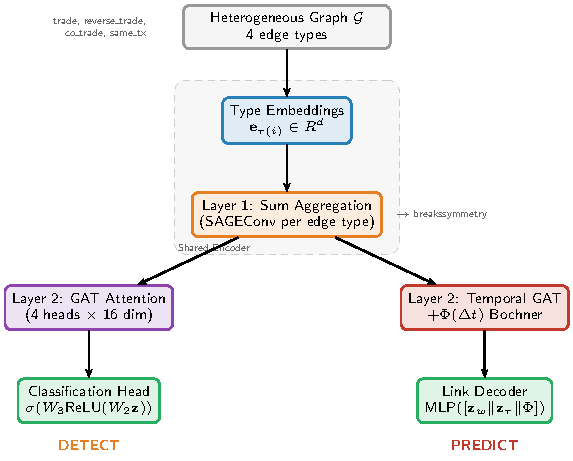
\includegraphics[width=\linewidth]{figures/architecture.pdf}
\caption{Overview of the coordination detection pipeline. Wallet--token
interactions are encoded as a heterogeneous graph with four edge types.
The featureless HeteroGAT (left) detects coordination retrospectively;
the temporal extension (right) predicts where coordinators will target next.}
\label{fig:architecture}
\end{figure}

\subsection{Coordination-Aware Architecture}
\label{sec:architecture}

The featureless HeteroGAT has ${\sim}69$K parameters. Each node
receives a learnable type embedding
$\mathbf{h}_i^{(0)}=\mathbf{e}_{\tau(i)}\in\mathbb{R}^{d}$ ($d{=}64$).
No other input is provided; the model must infer coordination
entirely from graph topology.

\smallskip\textbf{Proposition (GAT degeneracy).}
\textit{If $\mathbf{h}_j^{(0)}{=}\mathbf{c}$ for all $j$ of the same
type, then the GAT attention coefficients~\eqref{eq:gat} reduce to
$\alpha_{ij}^{(r)}=1/|\mathcal{N}_r(i)|$ for every neighbour $j$.}

\smallskip\textit{Proof sketch.}
With identical inputs, $\mathbf{W}_r\mathbf{h}_j^{(1)}{=}\mathbf{W}_r\mathbf{c}$
for all $j$, so $\mathbf{a}_r^\top[\mathbf{W}_r\mathbf{c}\|\mathbf{W}_r\mathbf{c}]$
is a constant independent of $j$. The softmax over identical logits
yields $\exp(e)/\sum\exp(e) = 1/|\mathcal{N}_r(i)|$, and attention
becomes uniform averaging, equivalent to mean
pooling~\cite{brody2022gatv2}. All degree information is discarded.

\smallskip
We resolve this with a two-stage \emph{sum-then-attention} design.
Layer~1 uses sum aggregation~\cite{hamilton2017graphsage} to encode
coordination degree:
\begin{equation}
  \mathbf{h}_i^{(1)} = \mathrm{ELU}\!\Bigl(
    \mathrm{LN}\!\Bigl(\sum_{r}\sum_{j\in\mathcal{N}_r(i)}
    \mathbf{W}_r^{(1)}\,\mathbf{h}_j^{(0)}\Bigr)\Bigr),
  \label{eq:sage}
\end{equation}
where $\mathbf{W}_r^{(1)}\!\in\!\mathbb{R}^{d\times d}$ ($d{=}64$),
$r$ indexes edge type, and LN denotes LayerNorm. A token traded by 100
wallets now has embedding magnitude $100\times$ that of one traded by a
single wallet, encoding the scale of coordination activity.

Layer~2 applies multi-head GAT attention~\cite{velickovic2018gat}
(4~heads, 16~dims each) on the now-differentiated nodes:
\begin{equation}
  \alpha_{ij}^{(r)} = \frac{
    \exp\!\bigl(\mathrm{LReLU}(\mathbf{a}_r^\top
    [\mathbf{W}_r\mathbf{h}_i^{(1)} \| \mathbf{W}_r\mathbf{h}_j^{(1)}])\bigr)
  }{
    \sum_{k\in\mathcal{N}_r(i)} \exp\!\bigl(\mathrm{LReLU}(\mathbf{a}_r^\top
    [\mathbf{W}_r\mathbf{h}_i^{(1)} \| \mathbf{W}_r\mathbf{h}_k^{(1)}])\bigr)
  }.
  \label{eq:gat}
\end{equation}
Messages from different edge types arriving at the same node are
aggregated by summation:
\begin{equation}
  \mathbf{z}_i = \mathrm{ELU}\!\Bigl(
    \sum_{r \in \mathcal{R}} \sum_{j\in\mathcal{N}_r(i)}
    \alpha_{ij}^{(r)}\, \mathbf{W}_r^{(2)}\mathbf{h}_j^{(1)}\Bigr)
    + \mathbf{h}_i^{(1)},
  \label{eq:hetero_agg}
\end{equation}
where the residual connection preserves the degree-differentiated
representations from Layer~1. The summation over edge types is a
deliberate design choice: it allows the attention mechanism within
each relation to weight individual neighbours, while preserving the
additive contribution of each coordination channel: a wallet
receiving both co-trading and same-tx messages accumulates evidence
from both sources. A two-layer MLP ($64\to32\to1$) produces token-level predictions
$\hat{y}_i = \sigma(W_3\,\mathrm{ReLU}(W_2\,\mathbf{z}_i^{\text{tok}}))$.
Training minimises the weighted binary cross-entropy:
\begin{equation}
  \mathcal{L}_{\text{cls}} = -\frac{1}{N}\sum_{i=1}^{N}\bigl[
    w_+\,y_i\log\hat{y}_i + (1{-}y_i)\log(1{-}\hat{y}_i)\bigr],
  \label{eq:bce}
\end{equation}
where $w_+{=}n_{\text{neg}}/n_{\text{pos}}{\approx}0.26$ down-weights
the majority high-risk class. We use AdamW ($\text{lr}{=}10^{-3}$,
$\text{wd}{=}10^{-3}$), cosine annealing ($T_{\max}{=}300$), gradient
clipping (max norm~1.0), and early stopping (patience 30 on validation
AUC). The model reaches peak validation AUC\,=\,0.856 at epoch~28;
training loss continues to decrease thereafter while validation
plateaus, the classic overfitting signature. Early stopping terminates
at epoch~58; inference over the full test graph completes in
$<$1\,s, confirming the model's suitability for deployment.

We also train a featured variant that replaces type
embeddings with MLP projections of the raw features (token:
$116\to64\to64$; wallet: $15\to64\to64$), keeping the same architecture
(${\sim}86$K parameters), to isolate the contribution of features on
top of topology. Table~\ref{tab:params} details the parameter budget.

\begin{table}[t]
\caption{Parameter count by component for both model variants.}
\label{tab:params}
\centering\small
\begin{tabular}{lrr}
\toprule
Component & Featureless & Featured \\
\midrule
Type/Feature embeddings & 128  & 16{,}640 \\
SAGEConv L1 ($4$ edge types) & 33{,}024 & 33{,}024 \\
GATConv L2 ($4\times4$ heads) & 33{,}792 & 33{,}792 \\
Prediction head ($64\to32\to1$) & 2{,}113 & 2{,}113 \\
\midrule
\textbf{Total} & \textbf{69{,}057} & \textbf{85{,}569} \\
\bottomrule
\end{tabular}
\end{table}

\subsection{Temporal Extension}
\label{sec:temporal}

Having shown that topology detects coordination retrospectively, we
now ask whether it can predict where coordinators will target next.
The temporal model retains the same two-layer structure (Layer~1
SAGEConv, $\mathbb{R}^{128}\to\mathbb{R}^{128}$, sum aggregation,
followed by Layer~2 attention) but replaces the static GAT in Layer~2
with a \emph{temporal} attention mechanism that conditions on the
time gap between interactions (${\sim}314$K parameters total).
Specifically, we augment the attention with a Bochner time
encoding~\cite{xu2020tgat}. For each edge with time gap
$\Delta t = (t_{\text{query}} - t_{\text{edge}})/86400$ (normalised
to days):
\begin{equation}
  \Phi(\Delta t) = \frac{1}{\sqrt{d_\Phi}}
    \bigl[\cos(\omega_1\Delta t + b_1),\ldots,
    \cos(\omega_{d_\Phi}\Delta t + b_{d_\Phi})\bigr],
  \label{eq:bochner}
\end{equation}
where $\omega_k, b_k$ are learnable ($d_\Phi{=}64$). The construction
follows from Bochner's theorem~\cite{rahimi2007random}: any
shift-invariant positive-definite kernel $k(\Delta t)$ admits a
spectral representation
$k(\Delta t)=\mathbb{E}_\omega[\cos(\omega\Delta t)]$, so the inner
product $\langle\Phi(t_1),\Phi(t_2)\rangle$ approximates a valid
temporal kernel. Making frequencies learnable lets the model discover
task-relevant timescales automatically~\cite{xu2020tgat}.

The temporal attention logits incorporate this encoding:
\begin{equation}
  e_{ij}^{(r)} = \frac{\mathrm{LReLU}\bigl(\mathbf{a}_r^\top
    [\mathbf{W}_s\mathbf{h}_i \| \mathbf{W}_d\mathbf{h}_j \|
    \Phi(\Delta t_{ij})]\bigr)}{\sqrt{2d+d_\Phi}}.
  \label{eq:temporal_attn}
\end{equation}

For a candidate interaction $(w,\tau)$ at time $t$, the decoder scores:
\begin{equation}
  \hat{y}_{w\tau}(t) = \sigma\!\bigl(\text{MLP}([\mathbf{z}_w \|
    \mathbf{z}_\tau \| \Phi(t{-}t_w^{\text{last}}) \|
    \Phi(t{-}t_\tau^{\text{last}})])\bigr),
  \label{eq:decoder}
\end{equation}
where $\mathbf{z}_w, \mathbf{z}_\tau$ are node embeddings after two
layers of temporal HeteroGAT. For each observed edge $(w,\tau^+,t)$ we
sample $K{=}19$ negative destinations $\{\tau_k^-\}$ uniformly at random
and minimise the binary cross-entropy:
\begin{equation}
  \mathcal{L}_{\text{link}} = -\log\hat{y}_{w\tau^+}
    - \frac{1}{K}\sum_{k=1}^{K}\log(1-\hat{y}_{w\tau_k^-}),
  \label{eq:link_loss}
\end{equation}
following the fixed negative sampling protocol
of~\cite{poursafaei2022edgebank}. The model has ${\sim}314$K parameters
(265K encoder + 49K decoder).

\subsection{Baselines and Evaluation}
\label{sec:baselines}

For classification, we compare against five feature-based models
operating on the 116 cleaned token features. The \emph{null baseline}
is L2-regularised logistic regression with balanced class weights, the
simplest linear model that preserves all input features and provides a
lower bound on learnable signal. We also evaluate SVM with RBF kernel,
Random Forest (200 trees), Gradient Boosting (200 estimators), and MLP
($116\to256\to128\to1$, ${\sim}64$K parameters). For link prediction,
we compare against three baselines: (i)~a random baseline (expected
MRR\,$\approx$\,0.180 for 20 candidates),
(ii)~EdgeBank~\cite{poursafaei2022edgebank} (memorises training edges
and predicts repeats), and (iii)~a most-popular-token heuristic that
ranks candidates by normalised training frequency. All reported metrics are
evaluated out-of-sample on the held-out week-52 test set unless
otherwise noted.

Classification metrics: AUC-ROC (primary), F1, AP, precision, and
recall, with 95\,\% bootstrap confidence intervals ($n{=}1{,}000$) and
McNemar's test for pairwise significance. Link prediction uses Mean
Reciprocal Rank and Hits@$K$:
\begin{equation}
  \text{MRR} = \frac{1}{N}\sum_{i=1}^{N}\frac{1}{\text{rank}_i},
  \quad
  \text{Hits@}K = \frac{1}{N}\sum_{i=1}^{N}\mathbb{1}[\text{rank}_i \leq K],
  \label{eq:mrr}
\end{equation}
where $\text{rank}_i$ is the position of the true destination among
$1{+}K_{\text{neg}}$ candidates (1 positive $+$ 19 negatives).

Algorithm~\ref{alg:pipeline} summarises the full pipeline.

\begin{algorithm}[t]
\caption{Coordination Detection Pipeline}
\label{alg:pipeline}
\DontPrintSemicolon
\KwIn{Weekly parquet files $\mathcal{D}_{\text{train}},
\mathcal{D}_{\text{val}}, \mathcal{D}_{\text{test}}$;
feature matrix $\mathbf{X}$; labels $\mathbf{y}$}
\KwOut{Trained models, predictions, evaluation metrics}
\BlankLine
\tcc{Phase 1: Graph construction}
\ForEach{split $s \in \{\text{train, val, test}\}$}{
  Load transactions $\mathcal{T}_s$ from parquets\;
  Build wallet$\to$token edges from $\mathcal{T}_s$\;
  Compute temporally-decayed co-trade edges (Eq.~\ref{eq:cotrade})\;
  Extract same-transaction edges\;
  Assemble $\mathcal{G}_s$ as PyG \texttt{HeteroData}\;
}
Z-score normalise features (fit on train)\;
\BlankLine
\tcc{Phase 2: Coordination detection (classification)}
Initialise FeaturelessHeteroGAT (Eqs.~\ref{eq:sage}--\ref{eq:gat})\;
$w_+ \gets n_{\text{neg}} / n_{\text{pos}} \approx 0.26$ \tcp*{class weight}
\For{epoch $= 1, \ldots, 300$}{
  $\hat{\mathbf{y}} \gets$ forward pass on $\mathcal{G}_{\text{train}}$\;
  $\mathcal{L} \gets \text{BCE}(\hat{\mathbf{y}}, \mathbf{y};\; \text{pos\_weight}{=}w_+)$\;
  Update via AdamW, cosine annealing, grad clip 1.0\;
  \If{val AUC not improved for 30 epochs}{\textbf{break}}
}
\BlankLine
\tcc{Phase 3: Coordination prediction (link prediction)}
Extract chronological events $(w, \tau, t)$ from $\mathcal{T}_{\text{train}}$\;
Encode $\mathcal{G}_{\text{train}}$ with temporal HeteroGAT (Eqs.~\ref{eq:bochner}--\ref{eq:temporal_attn})\;
\For{each batch of events}{
  Sample 19 negative tokens per positive\;
  Score via link decoder (Eq.~\ref{eq:decoder})\;
  $\mathcal{L} \gets \text{BCE}(\text{pos scores}, \text{neg scores})$\;
  Update decoder parameters\;
}
\BlankLine
\tcc{Phase 4: Evaluation}
Compute AUC, F1, AP with 95\% bootstrap CIs\;
Compute MRR, Hits@$K$ for link prediction\;
Run early detection at $h \in \{1, 6, 24, 72, 168\}$ hours\;
\end{algorithm}

% ====================================================================
\section{Results}
\label{sec:results}
% ====================================================================

\subsection{Coordination Detection}
\label{sec:classification_results}

Table~\ref{tab:results} reports test-set classification performance.
The featureless HeteroGAT (AUC\,=\,0.867) outperforms all five tabular
baselines despite using zero hand-crafted features, demonstrating that
graph topology alone encodes coordination signals that 116 engineered
features approximate imperfectly. When topology and features are
combined, the featured HeteroGAT reaches the highest overall score
(AUC\,=\,0.916). Decomposing this gain is instructive: adding graph
structure to features yields $\Delta\text{AUC}{=}+0.061$ (RF
0.855\,$\to$\,featured 0.916), whereas adding features to topology
yields only $\Delta\text{AUC}{=}+0.049$ (featureless
0.867\,$\to$\,featured 0.916). Graph structure therefore contributes
more marginal discriminative power than 116 engineered features.

These performance differences are not attributable to sampling
variance: McNemar's test confirms significance for the featureless
HeteroGAT against all individually tested baselines---logistic
regression
($\chi^2{=}13.6$, $p{<}0.001$), MLP ($\chi^2{=}7.2$, $p{=}0.007$),
and Random Forest ($\chi^2{=}7.3$, $p{=}0.007$). The featureless model's optimal
threshold is 0.79, compared to 0.09 (LogReg) and 0.13 (MLP),
indicating well-calibrated probabilities.

\smallskip\textbf{Error analysis.}
False negatives concentrate on tokens with fewer than five connected
wallets, where the coordination subgraph is too sparse for two-hop
message passing. False positives arise on organically popular tokens
whose high connectivity mimics coordinated structure. The
79\,\% high-risk base rate makes threshold-invariant AUC-ROC the
appropriate primary metric.

\begin{table*}[t]
\caption{Test-set classification performance (week~52). All models use the same chronological train/val/test split.
All models report 95\,\% bootstrap CI ($n{=}1{,}000$). Best result per column in bold. The graph-based models
(bottom) use heterogeneous message passing over four edge types; the featureless variant receives
zero hand-crafted features.}
\label{tab:results}
\centering
\begin{tabular}{llccccccc}
\toprule
& Model & Features & Parameters & AUC-ROC & F1 & AP & Precision & Recall \\
\midrule
\multirow{5}{*}{\rotatebox{90}{\scriptsize Tabular}}
& Logistic Regression & 116 & --- & .841\,[.825,\,.857] & .887 & .955 & .812 & \textbf{.977} \\
& SVM (RBF kernel) & 116 & --- & .834\,[.817,\,.849] & .805 & .953 & \textbf{.942} & .703 \\
& Random Forest & 116 & --- & .855\,[.840,\,.870] & .878 & .960 & .864 & .893 \\
& Gradient Boosting & 116 & --- & .849\,[.835,\,.863] & .878 & .959 & .865 & .890 \\
& MLP & 116 & 64K & .850\,[.835,\,.865] & .890 & .958 & .827 & .963 \\
\midrule
\multirow{2}{*}{\rotatebox{90}{\scriptsize Graph}}
& FeaturelessHeteroGAT$^*$ & 0 & 69K & .867\,[.852,\,.882] & .899 & .960 & .870 & .931 \\
& FeaturedHeteroGAT & 131$^\ddagger$ & 86K & \textbf{.916}\,[.905,\,.926] & \textbf{.918} & \textbf{.977} & .909 & .927 \\
\bottomrule
\multicolumn{9}{l}{\scriptsize $^*$Across seeds $\{42, 123, 7\}$: AUC\,=\,$0.869 \pm 0.002$, confirming training stability.}\\
\multicolumn{9}{l}{\scriptsize $^\ddagger$116 token + 15 wallet features.}
\end{tabular}
\end{table*}

\subsection{Edge-Type Ablation}
\label{sec:ablation}

The featureless model's reliance on topology raises a natural
follow-up: which edge types carry the coordination signal? To answer
this, we ablate the graph by removing one edge type at a time and
retraining from scratch (Table~\ref{tab:ablation}).

Same-transaction edges are the dominant coordination signal: removing
them drops AUC by 0.047 (from 0.867 to 0.820), a 5.4\% relative
decrease. This is consistent with same-tx edges encoding the strongest
form of coordination, wallets literally transacting within a single
atomic operation. By contrast, removing co-trading edges has negligible
impact ($\Delta\text{AUC}{=}+0.001$), suggesting that the temporal
co-trading signal is largely redundant with information already captured
by the bipartite trading structure. Even removing \emph{all}
wallet--wallet edges produces only a 0.004 AUC drop, indicating
that the bipartite wallet$\to$token$\to$wallet message-passing path
recovers most coordination information indirectly.

\begin{table}[t]
\caption{Edge-type ablation: featureless HeteroGAT retrained on
restricted graphs. Same-tx edges are the critical coordination signal.}
\label{tab:ablation}
\centering\small
\begin{tabular}{lccc}
\toprule
Configuration & AUC & $\Delta$ & AP \\
\midrule
Full graph (4 types)       & .867 & ---     & .960 \\
$-$ co-trade edges         & .868 & +.001   & .961 \\
$-$ all coordination (W-W) & .863 & $-.004$ & .958 \\
$-$ same-tx edges          & .820 & $-.047$ & .929 \\
\bottomrule
\end{tabular}
\end{table}

\subsection{Coordination Prediction}
\label{sec:link_results}

Having established that topology detects coordination, we now ask
whether it can predict where coordinated wallets will converge next.
Table~\ref{tab:link} reports link prediction performance, where both
heuristic baselines perform \emph{worse than random}.
EdgeBank~\cite{poursafaei2022edgebank} (MRR\,=\,0.056) fails because
meme-token trading is novelty-driven: wallets constantly interact with
new tokens rather than revisiting past ones, so memorising historical
edges is actively misleading. The popularity baseline
(MRR\,=\,0.056) fails because insider coordination targets niche
tokens, not popular ones.
A cosine-similarity baseline using the same frozen embeddings achieves
MRR\,=\,0.250, confirming that the temporal decoder contributes
substantially beyond static embedding proximity.
The temporal HeteroGAT achieves
MRR\,=\,0.490 ($2.7\times$ random, ${\sim}8.8\times$ EdgeBank), placing the
true next token at rank ${\sim}$2 on average among 20 candidates.
Hits@10\,=\,0.952 means the true token is in the top half 95\,\% of
the time. These results confirm that the temporal model learns
structural coordination patterns, specifically which wallet clusters
converge on which tokens, rather than exploiting recurrence or
popularity.

\begin{table}[t]
\caption{Temporal link prediction (within-week validation, 1~positive
+ 19~negatives per query). EdgeBank~\cite{poursafaei2022edgebank}
memorises training edges; Popularity ranks by token frequency.
Both heuristics score below random, confirming that the temporal
model learns coordination patterns rather than recurrence or
popularity.}
\label{tab:link}
\centering\small
\begin{tabular}{lcccc}
\toprule
Model & MRR & Hits@1 & Hits@3 & Hits@10 \\
\midrule
Random & .180 & .050 & .150 & .500 \\
EdgeBank & .056 & .005 & .007 & .009 \\
Popularity & .056 & .002 & .005 & .024 \\
Cosine Sim. & .250 & .078 & .268 & .695 \\
Temporal HeteroGAT & \textbf{.490} & \textbf{.296} & \textbf{.581} & \textbf{.952} \\
\bottomrule
\end{tabular}
\end{table}

These results have a direct operational consequence: predicted
convergence of wallets historically associated with manipulation
constitutes an early warning that retrospective classification cannot
provide, bridging the temporal gap identified in
Section~\ref{sec:early}. The learnable Bochner frequencies adapt to
Solana coordination timescales (sub-minute bundling, hourly organic
cycles, daily rhythms) without manual specification. The reported MRR
of 0.490 uses frozen GNN embeddings and is therefore a lower bound on
temporal predictive capacity.

\subsection{Signal Emergence}
\label{sec:early}

A deployment-critical question is how quickly topological signal
becomes useful. We evaluate the featureless HeteroGAT on subgraphs
containing only edges from the first $h$ hours of the test week;
tabular baselines use features computed from the full week and are
therefore time-invariant upper bounds (Table~\ref{tab:early}).

At 1\,hour (0.1\,\% of edges), coordination structure is too sparse
for the GNN (AUC\,=\,0.500). Signal emerges at 24\,hours (0.542,
8\,\% of edges) and strengthens at 3\,days (0.611, 34\,\%), the
critical mass at which two-hop coordination paths become
distinguishable from chance. At 7\,days the GNN converges to
AUC\,=\,0.841. Feature-based methods provide immediate signal;
graph topology requires edge accumulation but converges without
feature engineering. A practical system would combine both: tabular
features for instant screening, augmented by evolving graph
structure---where the link predictor
(Section~\ref{sec:link_results}) bridges the accumulation gap.

\begin{table}[t]
\caption{Early detection: classification AUC as a function of
observation time. Tabular baselines use full-week features (upper bound).}
\label{tab:early}
\centering\small
\begin{tabular}{lccccc}
\toprule
Model & 1h & 6h & 24h & 3d & 7d \\
\midrule
LogReg & .841 & .841 & .841 & .841 & .841 \\
RF     & .855 & .855 & .855 & .855 & .855 \\
Feat.less GAT & .500 & .500 & .542 & .611 & .841 \\
\% edges & 0.1 & 1 & 8 & 34 & 95 \\
\bottomrule
\end{tabular}
\end{table}


\subsection{Coordination Archetypes}
\label{sec:archetypes}

To examine whether the learned embeddings encode interpretable
structure, we apply HDBSCAN clustering~\cite{mcinnes2017hdbscan} to
the 64-dimensional wallet embeddings (minimum cluster size 50,
Euclidean distance), obtaining 25 clusters with only 2.1\,\% noise
despite no supervision on wallet types.

Three coordination archetypes emerge.
\textit{(a)~Tight, high-coordination wallets} (${\sim}$12\,\% of the
active population) exhibit narrow token focus and dense
same-transaction connectivity, consistent with automated bundler
operations~\cite{hu2026memetrans}. These wallets are
disproportionately linked to high-risk tokens (34\,\% of high-risk
connections vs.\ 12\,\% population share).
\textit{(b)~Broad, low-coordination wallets} (${\sim}$45\,\%) trade
across many tokens with minimal same-transaction overlap, interacting
with high-risk tokens at the population base rate (${\sim}$79\,\%),
consistent with organic retail behaviour.
\textit{(c)~Intermediate, loosely synchronised wallets} display
elevated temporal co-trading similarity but few same-transaction
edges---the ``soft coordination'' that the temporally-decayed
co-trading edges~(Eq.~\ref{eq:cotrade}) are designed to capture and
that same-transaction analysis alone would miss.

The separation between archetypes reinforces the classification and
prediction results: the coordination edges that drive detection and
prediction also produce semantically meaningful clusters, confirming
that the learned representations encode genuine coordination
structure rather than statistical artefacts.

% ====================================================================
\section{Discussion}
\label{sec:discussion}
% ====================================================================

The three experimental views---detection, prediction, and
characterisation---converge on a single conclusion: graph topology
functions as a coordination fingerprint. The featureless model's
superiority over all tabular baselines demonstrates that wallet--token
interaction topology directly encodes coordination signals that 116
engineered aggregate statistics can only approximate.

This claim warrants nuance. The AP scores are effectively identical
between the featureless model (0.960) and Random Forest (0.960),
indicating comparable positive-class ranking quality. The AUC-ROC
advantage ($+0.012$) reflects stronger discrimination in the low
false-positive-rate regime---where a monitoring system would operate,
since early warnings require high specificity. The more important
finding is the marginal contribution analysis: adding graph structure
to features yields $\Delta$AUC\,=\,+0.061, whereas adding features to
topology yields only $\Delta$AUC\,=\,+0.049. Topology and features
capture partially overlapping but distinct signals, and their
combination (AUC\,=\,0.916) substantially exceeds either alone.

The temporal extension further establishes that this fingerprint is
\emph{predictive}, not merely retrospective. The failure of
recurrence- and popularity-based heuristics---scoring below
chance---confirms genuine structural learning. The cosine-similarity
baseline (MRR\,=\,0.250 vs.\ temporal model's 0.490) isolates the
contribution of Bochner-encoded temporal attention: static embedding
proximity accounts for roughly half the signal, while time-aware
attention contributes the remainder by learning coordination
timescales. The sum-then-attention design is architecturally necessary:
standard GAT with identical embeddings reduces to mean pooling,
discarding degree information. This principle generalises to any
featureless GNN setting. The early-detection analysis establishes the
two modalities as complementary, defining a staged architecture in
which the link predictor bridges the initial accumulation period.

Several limitations qualify these findings: (i)~weekly snapshot
granularity that sacrifices intra-day dynamics, which continuous-time
models~\cite{xu2020tgat,rossi2020tgn,yu2023dygformer} could capture;
(ii)~a high positive rate (79\,\%) that inflates absolute metrics
while preserving relative comparisons;
(iii)~pre-computed GNN embeddings for link prediction that prevent
end-to-end gradient flow (MRR\,=\,0.490 is a lower bound); and
(iv)~only 28.8\,\% of test-week wallets appear in training---the
remaining 71.2\,\% receive identical type embeddings, discarding
historical reputation. \emph{Persistent wallet embeddings}, carrying
forward learned representations across weeks, would let the GNN
recognise returning coordinators immediately---integrating naturally
with TGN-style per-node memory~\cite{rossi2020tgn}. End-to-end
temporal training, cross-week stability analysis, and entity
resolution of co-clustered wallets remain as future directions.

Taken together, these findings establish that graph topology provides a
self-contained coordination signal: the featureless approach requires
only the public transaction ledger, making detection, prediction, and
characterisation accessible without proprietary data or feature
engineering infrastructure.

% ── Bibliography ───────────────────────────────────────────────────
{\footnotesize
\bibliographystyle{IEEEtran}
\bibliography{references}
}

\end{document}
